(by Ari Wahl)

For our Ergonomic Pose App "PoseFix" we will use YOLO v8 pose as a base model. 
It can run on mobile devices (Android and Os) with 6-7 frames per second \cite{ultralytics2022}, 
which is more than enough for our application as well as on laptops or desktop computers. For data protection and privacy we will send only the keypoints from the pose detection 
the be evaluated online on our classification layer or alternatively run the model as a lightweight application completely on the users devices. 
Either way, this ensures that there is no threat for businesses or private persons as customers to be victims of spy attacs. Just having keypoints 
would only allow for an extremely abstract representation and is therefore a perfect measure to protect the data and privacy of our customers. 
For the adaption of the YOLOv8 pose model for our application, we train a classification layer on basis of the keypoint representation. 
To evaluate, if a pose is ergonomic or not, we collected a dataset, which uses classification levels from the well established RULA (Rapid Upper Limb Assessment) employee assessment 
worksheed \cite{Holzgreve_2022}. 
Additional implementations that exceed the base model will be a dashboard for monitoring the posture over time and show long term improvements 
to the customer. Also we plan to optionally leverage Explainable AI methods to indicate which joint positions are problematic and show
 in which direction an improvement can be achieved most quickly. To establish more trust among our (potential) customers 
 we will also aim to get some certification(s) that prove the health impact of our application, e.g. TÜV. 
Our Technology is unique because we use a lightweight model that can run on mobile devices and laptops/desktops but will be implemented to achieve a high classification accuracy.
Its unique selling point is the userfriendlyness which provides a subtle user-interface as well as it optionally gives advice on how to change your posture.
So far we have not found any other application that provides a similar service.

\section{Mock-up}

For our mock-up we decided to use the traffic light colored-scheme that will be displayed as a frame. 
The frame will be green if the user's posture is correct, yellow if the posture is not optimal and should be changed soon and red if the posture is bad and should be changed immediately.
As you can see, a darker green is chosen, to make sure that the user is not distracted, if their posture is fine.
In the working setup, the user does not see their own image but instead the usul screen content. The feedback-frame will be displayed around the screen content. 
For the mock-up we will also show the keypoints our base model detected. The keypoints will be displayed as dots in the image. The user can choose if we will also provide a visual feedback in the form of a small window that will be displayed in the corner of the user's screen.
There it would then display the keypoint where the user's posture is bad and should be corrected in a different color than the other keypoints. 
In a more advanced state, we can also output an arrow in the image on how/which direction to correct the posture next to the highlighted parts.

\begin{figure}[ht]
    %\centering
    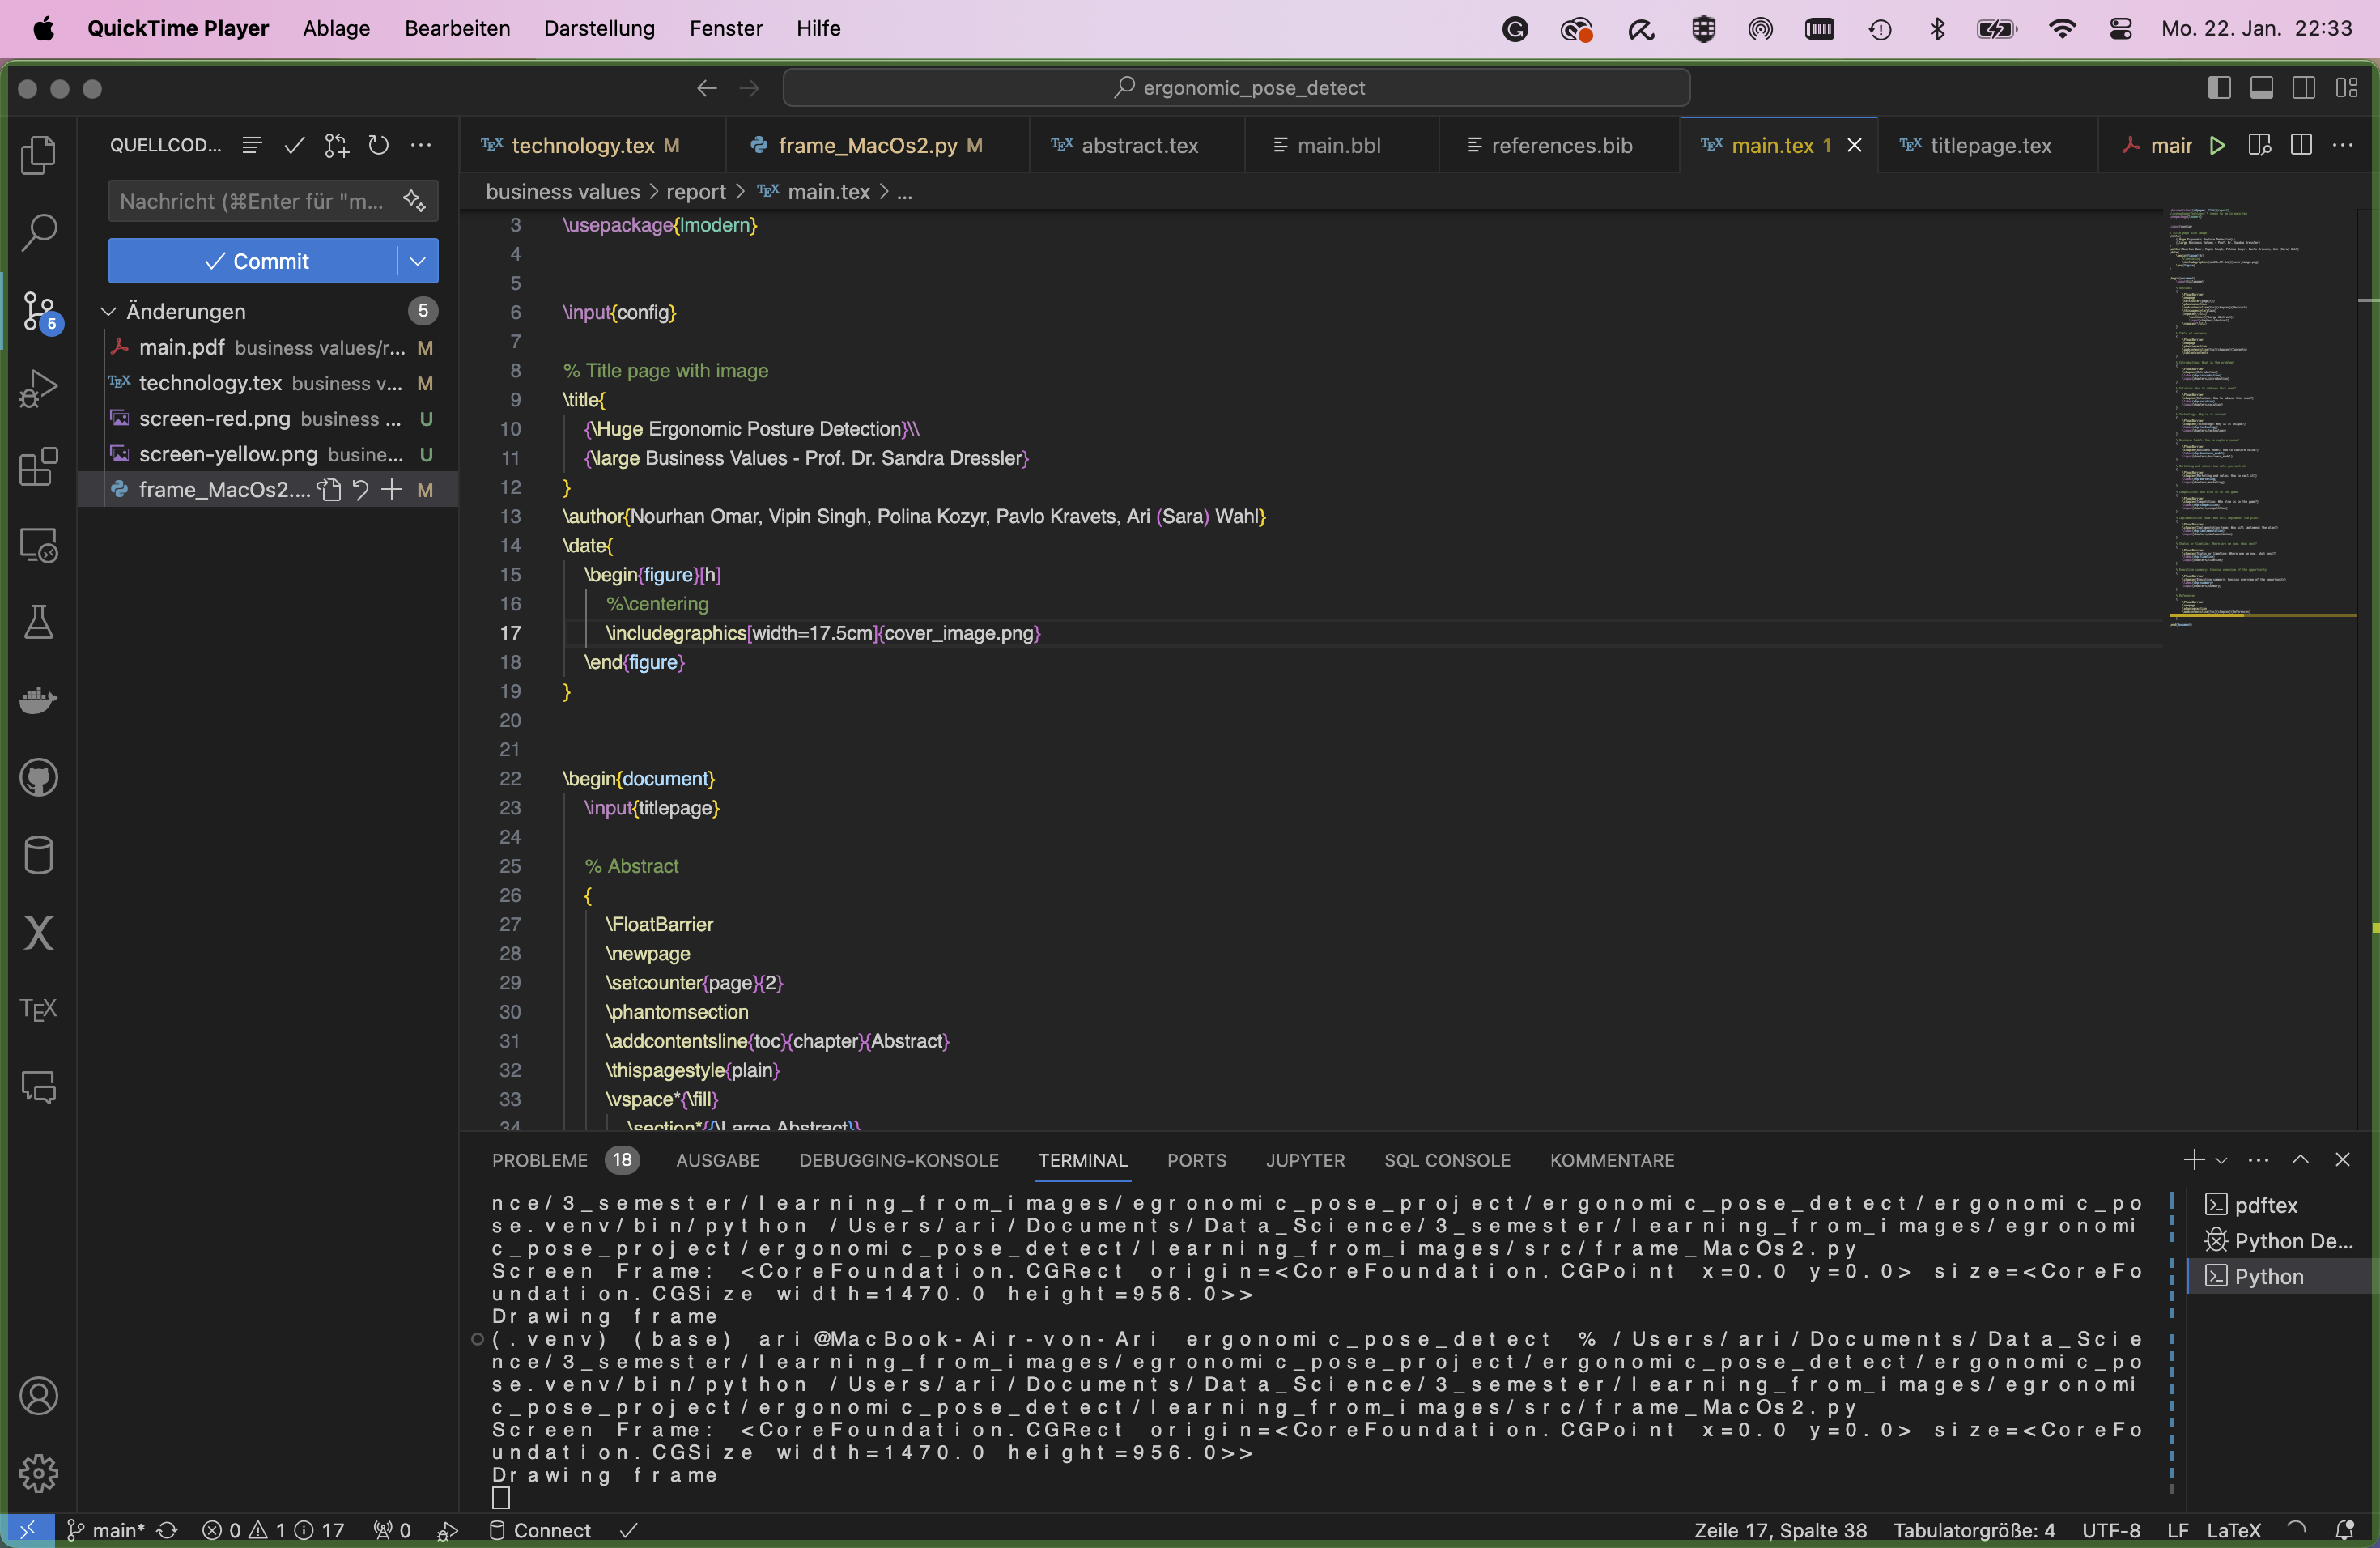
\includegraphics[width=15cm]{screen-green.png}
\end{figure}

\begin{figure}[ht]
    %\centering
    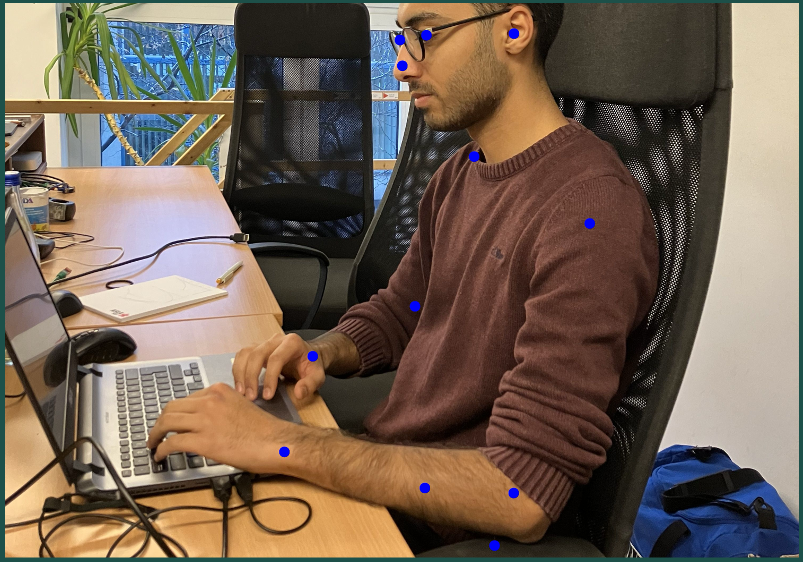
\includegraphics[width=15cm]{mock_up_green.png}
\end{figure}

\begin{figure}[ht]
    %\centering
    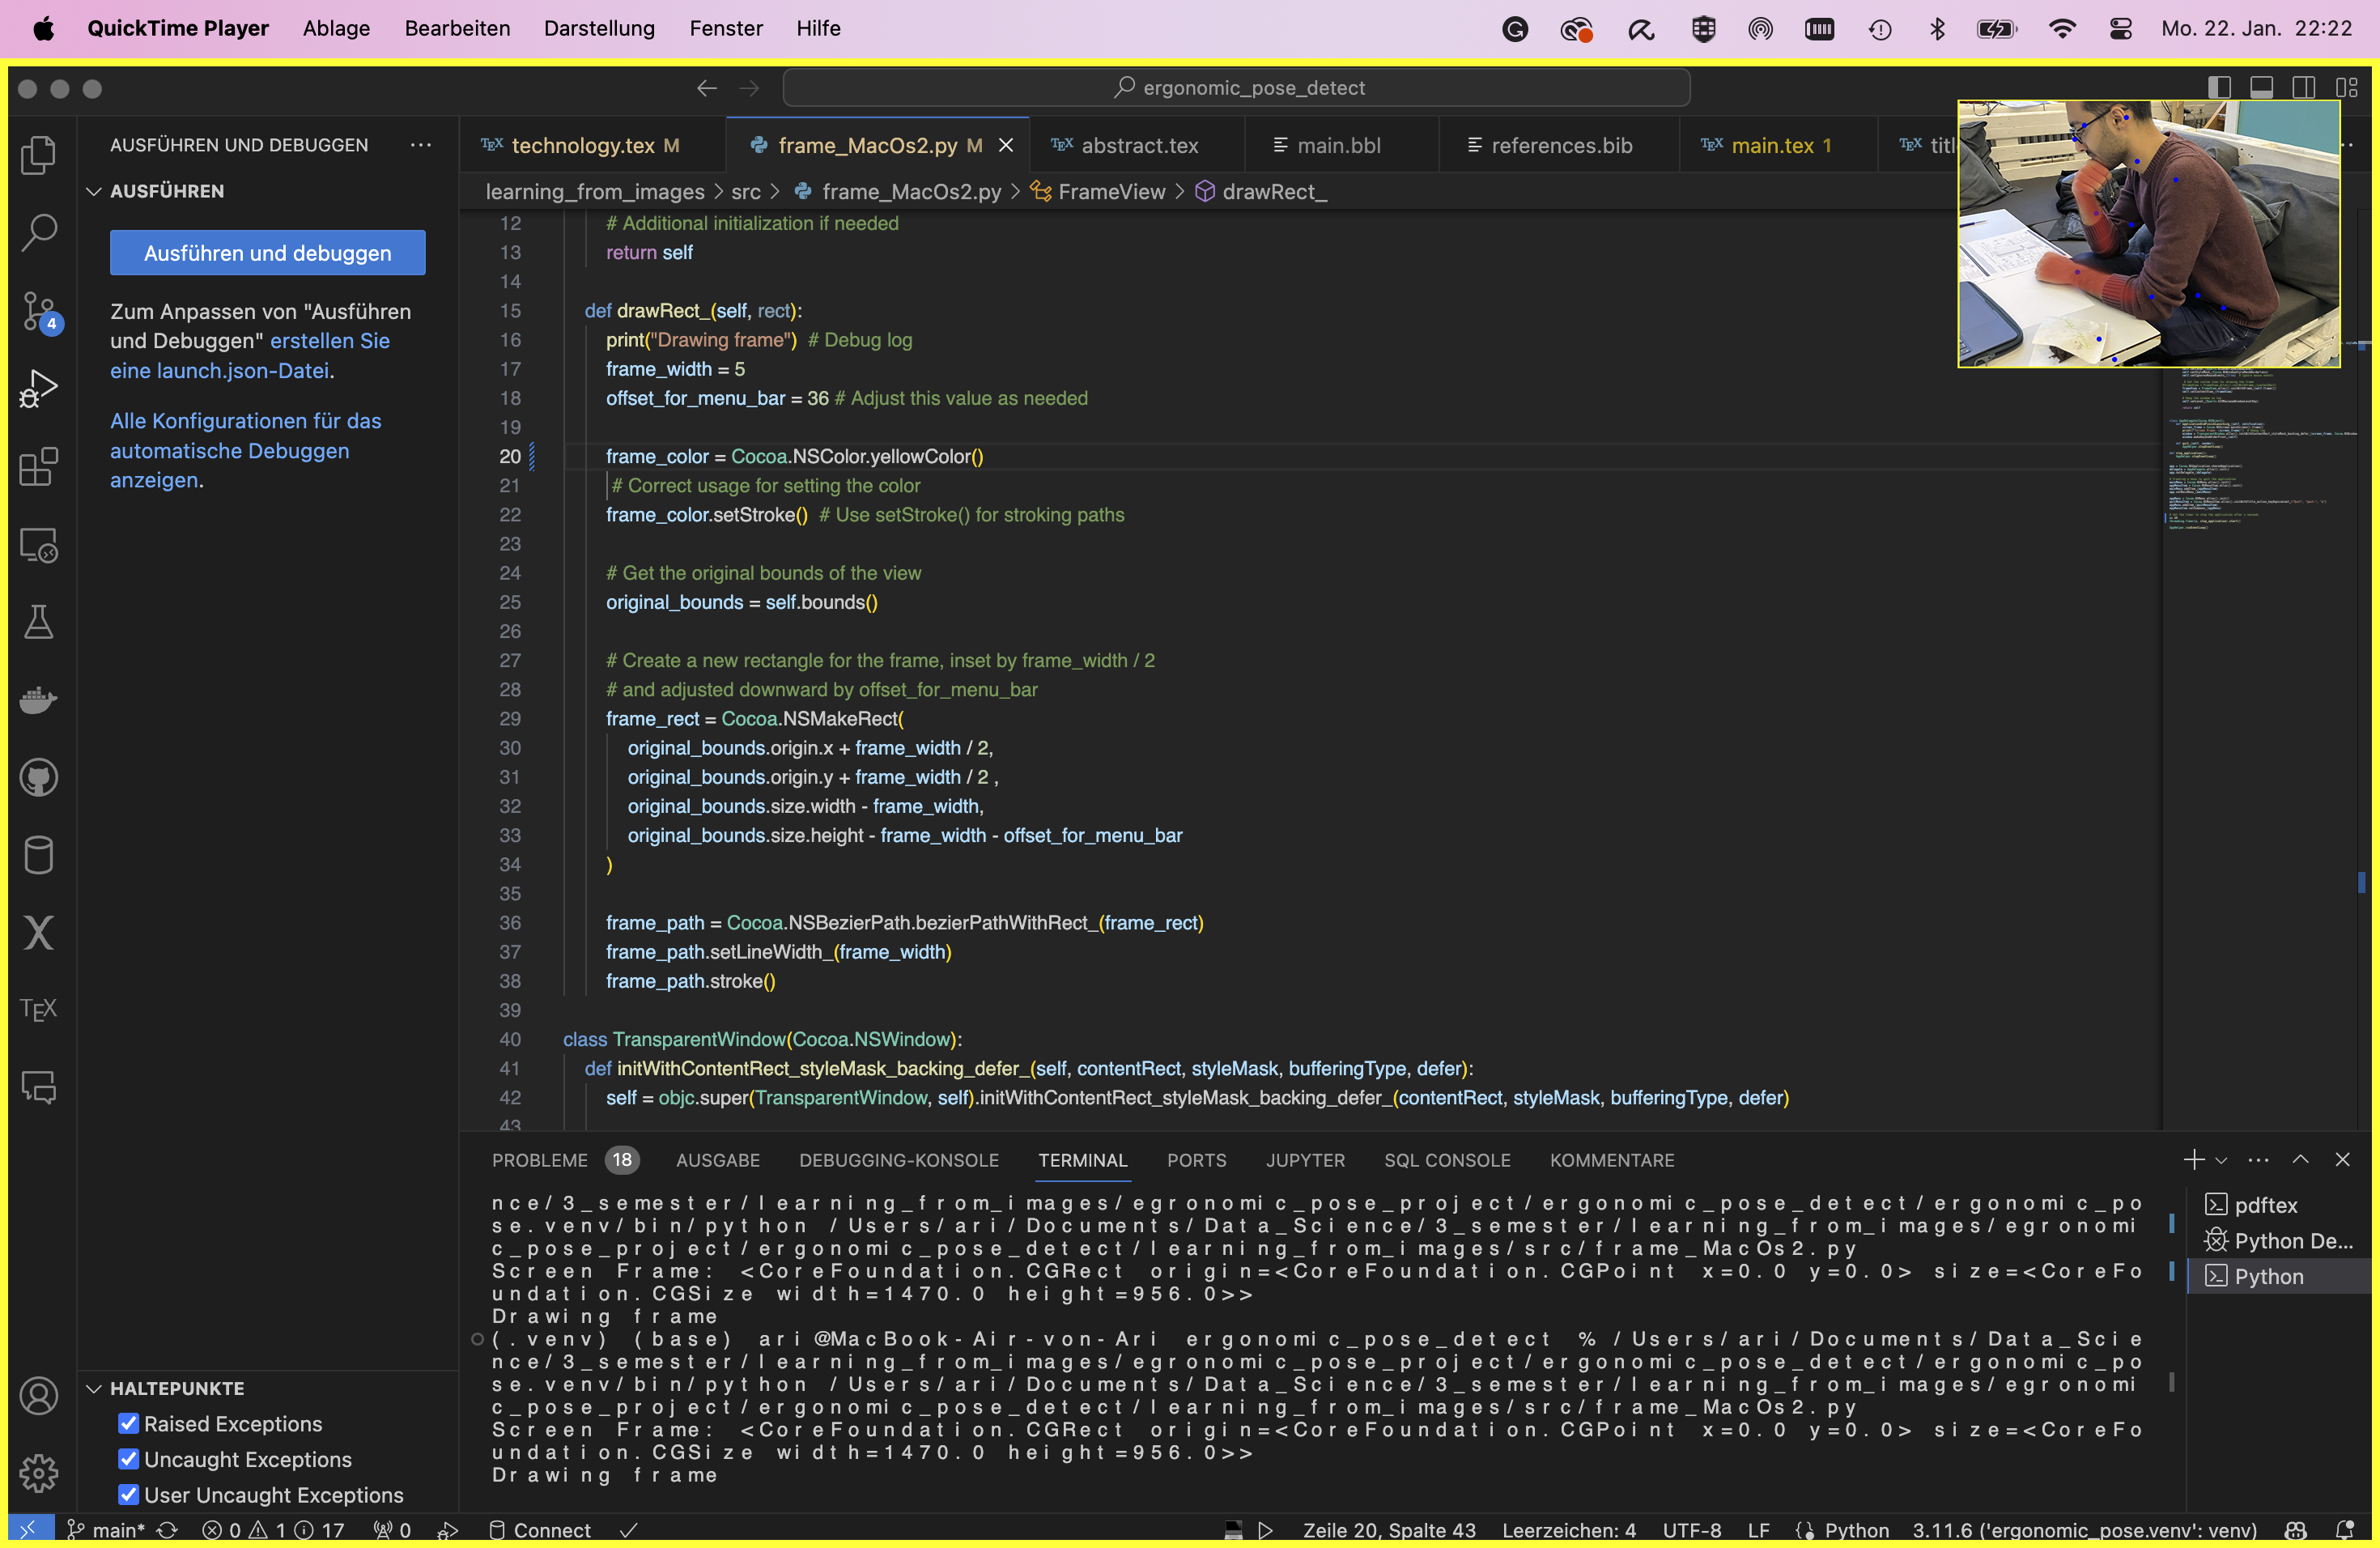
\includegraphics[width=15cm]{screen-yellow-mini_xai.png}
\end{figure}

\begin{figure}[ht]
    %\centering
    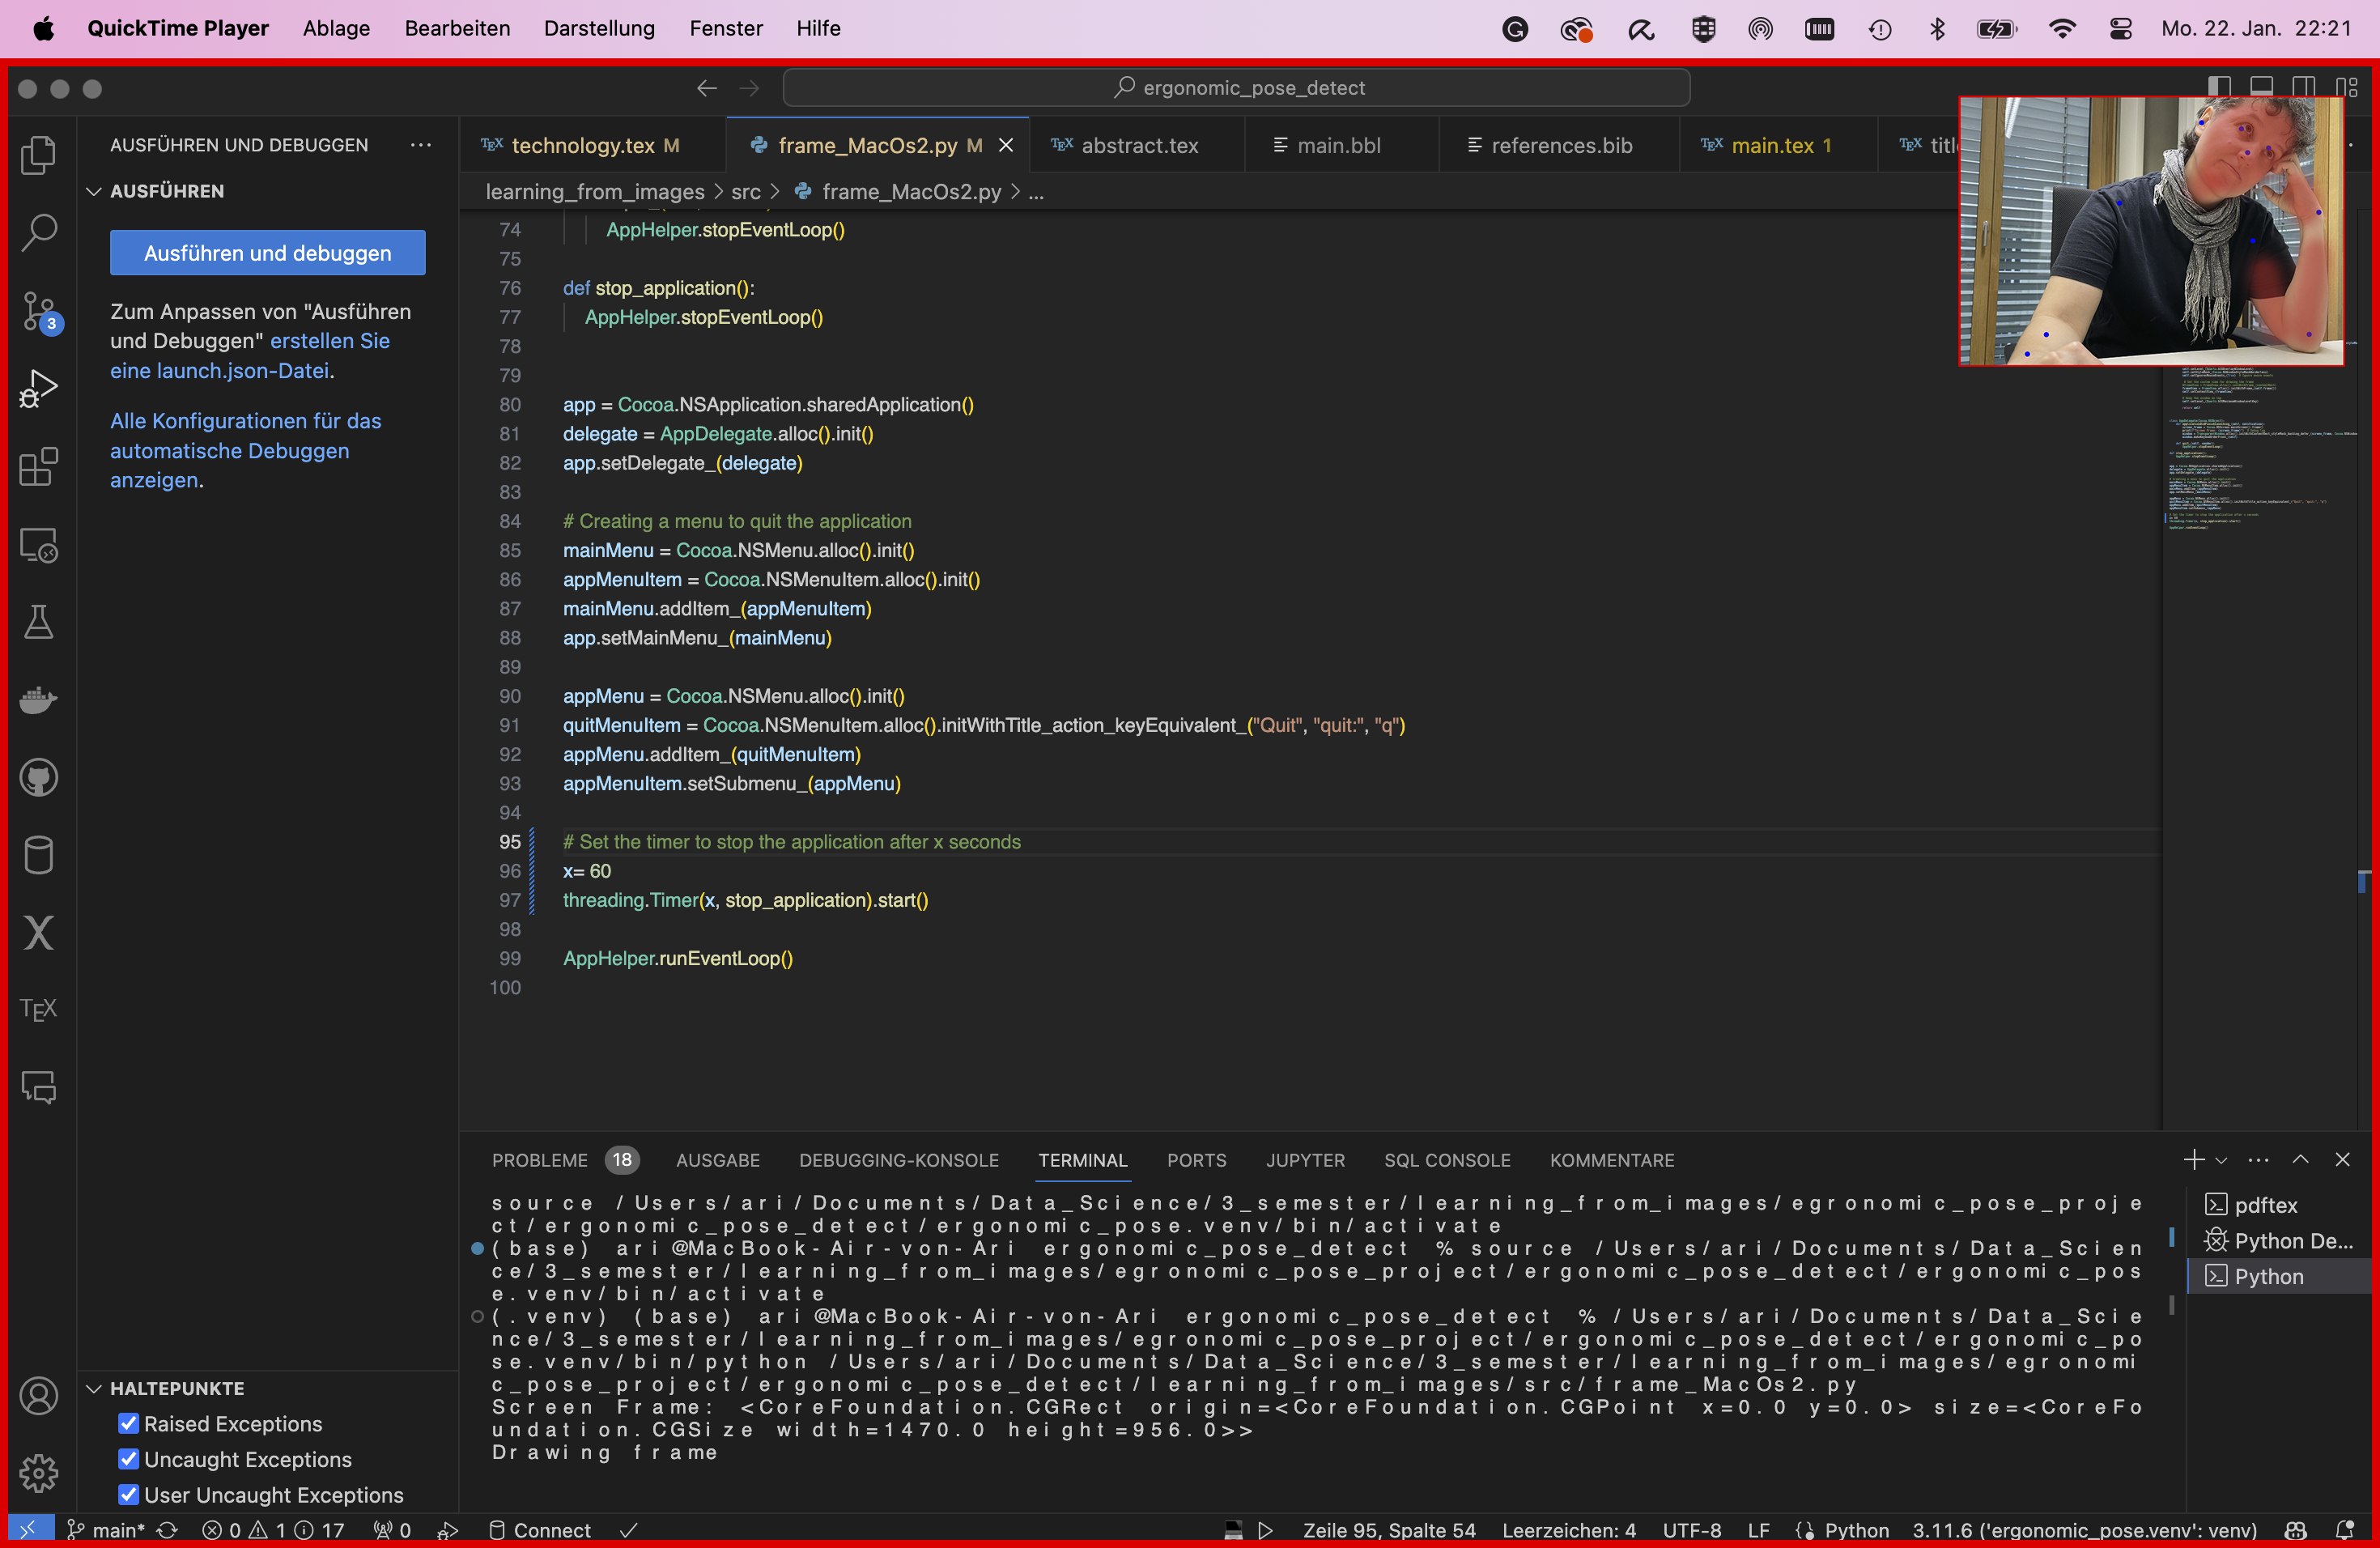
\includegraphics[width=15cm]{screen-red-mini-xai.png}
\end{figure}




\section{PEST-Analysis}

A PEST-analysis was done to evaluate the external factors that might influence our business. Since this includes political, economic, social and technological factors, 
and we focus on the technological factors in this chapter, we decided to include the PEST-analysis in this chapter. And since we are a startup, we also included a 
SWOT-analysis, that was informed by the PEST-analysis. 

\subsection{Political Factors}

\begin{itemize}
  \item \textbf{Labor Laws}:
  \begin{itemize}
    \item The Workplace Ordinance ArbStättV outlines employer responsibilities for ergonomic workplaces.
    \item Potential benefits from stricter ergonomic regulations for the B2B model \autocite{ArbStattV}.
  \end{itemize}

  \item \textbf{Data Privacy}:
  \begin{itemize}
    \item Compliance with the General Data Protection Regulation (GDPR) is vital for handling employee data \autocite{GDPR}.
  \end{itemize}

  \item \textbf{AI-Related Regulations}:
  \begin{itemize}
    \item The EU AI Act could affect the use and cost of third-party AI software \autocite{EUAIACT}. 
    Since movement patterns are as unique as fingerprints, our product may be labeled as a moderate or high-risk AI system, requiring additional certifications and meeting compliance requirements.
  \end{itemize}

  \item \textbf{Copyright Laws}:
  \begin{itemize}
    \item Importance of using copyright-free or properly licensed third-party software or pretrained models \autocite{CopyrightLaws} to save money and computantional effort. 
  \end{itemize}

  \item \textbf{Environment Laws}:
  \begin{itemize}
    \item In the future, AI products may be regulated due to their high energy consumption. Using pretrained models helps reducing the environmental cost.
  \end{itemize}

  \item \textbf{Opportunities and Risks}:
  \begin{itemize}
    \item Labor laws currently favor the B2B model, but future changes in ergonomic regulations pose risks.
    \item GDPR compliance offers appeal to privacy-conscious customers but incurs higher initial costs.
    \item Evolving AI and copyright laws present ongoing challenges and opportunities.
  \end{itemize}
\end{itemize}


\subsection{Economic factors}


\begin{itemize}
  \item \textbf{Return to Office Work}:
  \begin{itemize}
    \item Decreased remote work reduces demand in the B2C segment focused on home offices.
    \item Overall demand might diminish as employees working remotely often have dual workplace setups.
  \end{itemize}

  \item \textbf{Shift in Job Distribution}:
  \begin{itemize}
    \item A shift from desk jobs to manual labor initially challenges the business model.
    \item Potential long-term expansion into ergonomic solutions for manual labor sectors, requiring extensive training and data.
    \item Close monitoring of job distribution changes due to AI technology impacts is crucial for strategic planning.
  \end{itemize}

  \item \textbf{Economic Climate - Inflation}:
  \begin{itemize}
    \item High inflation rates could lead to reduced demand as businesses may limit investments.
  \end{itemize}
\end{itemize}

\subsection{Social factors}


\begin{itemize}
  \item \textbf{Changing Sensibilities Towards AI Monitoring}:
  \begin{itemize}
    \item Increasing desensitization to data privacy concerns, driven by widespread use of social media.
    \item Potential resistance to constant visual monitoring at the workplace, despite anonymized data.
    \item A shift towards greater privacy concern could necessitate investments in marketing and certifications for consumer assurance, impacting profitability.
  \end{itemize}

  \item \textbf{Social and Cultural Focus on Health}:
  \begin{itemize}
    \item Growing societal emphasis on health and quality of life aligns with the product's benefits.
    \item This trend supports both B2C and B2B demand, influenced by regulatory changes focusing on workplace health.
    \item Potential decline in demand if societal attitudes shift away from health focus.
  \end{itemize}

  \item \textbf{Demographic Considerations}:
  \begin{itemize}
    \item Aging workforce with existing health issues due to poor workplace ergonomics supports current demand.
    \item The impending mass retirement of the boomer generation could reduce long-term demand.
    \item Younger generations seeking more flexible work schedules and better work-life balance could also affect demand.
  \end{itemize}
\end{itemize}

\subsection{Technological factors}

\begin{itemize}
  \item \textbf{State of the Art Technology and Automation}:
  \begin{itemize}
    \item Current technology is advanced, reducing the immediate impact of technological changes.
    \item Ongoing research and development are crucial to stay ahead of emerging technologies that could enhance ergonomic predictions, data privacy, and AI efficiency.
  \end{itemize}

  \item \textbf{Continuous Innovation Strategy}:
  \begin{itemize}
    \item The goal is to maintain a state-of-the-art position in the market.
    \item Proactive adaptation to new developments to ensure they are not a threat to the business.
  \end{itemize}

  \item \textbf{Competition from Large Tech Companies}:
  \begin{itemize}
    \item Major risk from big tech companies potentially incorporating similar business ideas into their existing products, like operating systems or Microsoft 365 applications.
    \item Such integration by large companies could significantly and rapidly decrease the demand for the product.
  \end{itemize}
\end{itemize}

\section{SWOT-Analysis}

Our SWOT-Analysis was informed by the PEST-Analysis. It captures the internal strengths and weaknesses of our business model as well as the external opportunities and threats.

\begin{figure}[H]
    %\centering
    
\includegraphics[width=\textwidth]{SWOT_analysis.png}
    \caption{SWOT-Analysis for our business model} 
    \label{fig:swot}
\end{figure}


In the SWOT-Analysis \ref{fig:swot} the internal factors are strengths and weaknesses, 
while the external factors are opportunities and threats and the positive factors are strengths and opportunities, 
while the negative factors are weaknesses and threats.